% !TeX root = surgery.tex

\subsection{Manuscripts}
Our edition results from considering the textual evidence of three manuscripts, all of which were preserved and most likely produced in Nepal, in Kathmandu valley, to be more precise. \textcites[\S 
2.1]{kleb-2021b} furnishes a comprehensive description of the individual manuscripts, quotes and translates their colophons and thoroughly examines various problems involved in their interpretation. That is why we will present only the key data essential for the study of our edition in the present paper.
In referring to the manuscripts, we use the sigla K, N and H, which correspond to the initial letters in the names of the libraries and collection where the respective bundles were discovered.

\begin{description}
\item[Siglum K:] The MS has been preserved at the Kaiser Shamsher (KL) library in Kathmandu, accession number KL 699. It was microfilmed and catalogued by the NGMPP/ NGMCP as C 80-7.%
    \footnote{%
    See 
    \url{http://catalogue-old.ngmcp.uni-hamburg.de/mediawiki/index.php/C_80-7_Suśrutasaṃhitā}
     (accessed on October 22, 2021).%
    } 
The MS comprises 152 palm-leaf folios that originally belonged to several different codicological units written by different scribes.%
    \footnote{%
    \textcites[46]{bhat-2020} and \textcites[11]{kleb-2021b} agree that four to five scribes were involved in the manuscript's production.
    } 
The folios are 53.5 $\times$ 4.4 cm in size and have two string holes.  The text is written in the so-called transitional Gupta script, with six to eight lines per folio.%
    \footnote{%
    Codicological features of the manuscript, such as the layout, peculiarities of the script, various ornamental and text-dividing symbols and many more, were scrutinized in \textcites{bhat-2020}.
    }
The MS is incomplete and contains a large part of the \emph{Suśrutasaṃhitā} as well as the \emph{Suśrutanighaṇṭu}.%
    \footnote{%
    See \textcites[11]{kleb-2021b} for a detailed description of the content.%
    }
The date stated in the colophon at the end of the compendium is verified for Sunday, April 13, AD 878. However, some controversy is involved in interpreting the exact roles of two persona mentioned in the same concluding remarks, someone Śrī Harṣacandra and Vaidya Vasuvarman.
\textcites[16]{kleb-2021b} thinks that the former “either sponsored the copying enterprise or wrote the manuscript himself” and that he later “donated it to Vaidya Vasuvarman on the condition that he (Vasuvarman) would study the text and explain it to others. The second condition was that the manuscript should remain in the family and not be given away either for sale or as a pawn. If the manuscript sat unused, it should be returned to Śrī Harṣacandra.”%    
    \footnote{%
    See \textcites[13--17]{kleb-2021b} for a translation and a study of the colophon, as well as an exposition of different positions related to its interpretation.%
    }

\item[Siglum N:] This MS is kept at the National Archives Kathmandu (NAK), under accession number 1-1079 \dev{ka}. It was microfilmed twice by the NGMPP as A 45-5(1) and A 1267-11(2).%
    \footnote{%
See 
\url{http://ngmcp.fdm.uni-hamburg.de/mediawiki/index.php/A_45-5_(Suśrutasaṃhitā)}
 (accessed on October 22, 2021)/
    } 
The MS comprises 65 palm-leaf folios, 56 $\times$ 5 cm in size, with two string holes each, and it is bundled together in a composite manuscript with at least one other medical work. The text is written in a variety of Newari script, with ca.\ seven lines per folio. Although the text contained in the MS does not cover the entire \emph{Suśrutasaṃhitā} and breaks off abruptly in the second chapter of the \emph{śārīrasthāna}, the actual MS, as a codicological unit, appears complete, that is, no leaf seems to be missing from the originally unitary artefact. Based on paleographic considerations, the MS can be dated tentatively to the 12th or 13th century.

\item[Siglum H:] The MS belongs to the historical collection of Hemarāja Śarman (fl.\ 1878-1953) and is currently kept at the NAK under accession number NAK 5-333. It is microfilmed twice by the NGMPP as B 29-19 and B 30-15, but the latter microfilm is incomplete.%
    \footnote{%
    See 
    \url{http://ngmcp.fdm.uni-hamburg.de/mediawiki/index.php/B_29-19_Suśrutasaṃhitā}
     (accessed on October 22, 2022).
    } 
The MS comprises 435 palm-leaf folios, 34 $\times$ 5 cm in size, with one string-hole in the middle. It is written in a type of Newari script that is more recent than the one used in N, with approximately six lines per folio. The MS is exceptionally well-preserved and complete, containing the text of the \emph{Suśrutasaṃhitā} as well as the \emph{Suśrutanighaṇṭu}. The final colophon identifies the scribe of the MS as Vaidya Amarasiṃhaka, son of Kamaladatta, and states the date on which he concluded the copying of the text. Both reading, that is, deciphering the actual characters, and interpretation of the concerned passage involve diverging opinions, all of which concur, however, in assigning the MS to the 16th century. \textcites[21--26]{kleb-2021b} gives an analytical account of the views expressed in literature, considers further options and puts forward his understanding that the MS was completed on Sunday, July 29, AD 1543.  
\end{description}
  
\subsubsection{Features of the manuscript transmission}
Andrey
\subsubsection{Palaeographical features}
\begin{itemize}
    \item śrita for śṛta.
    \item yātri for yātṛ (Su.ka.1.63) % but yātrin is possible
     \item punarṇṇavā  (Su.ka.1.61) % but an old Nepelase ms. of the Brahmayāmala has this spelling.
    \item ś and s in KL 699.
    \item b and v in KL 699 and NAK 5-333.
    \item cha and ccha
    \item line-fillers
    \item \d n for n (punar\d n\d nav\=a)
    \item vyājī-kṛ for vājī-kṛ
\end{itemize}

\subsubsection{Chart of characters}

[[[Put a chart from QuickPalaeographer here.]]]

\subsection{The Printed Editions}

The careful survey of printed editions of the \SS\ by Meulenbeld lists no fewer than 
44 entries.\footcite[IIB, 311--314]{meul-hist}  These range from the first edition 
by 
Madhusūdana Gupta (\citeyear{gupt-1835}) to editions in the 1970s. The 
number of 
reprints and editions since that time might almost double that number.  
Translations begin with Hessler's Latin translation in \citeyear{hess-1855} and 
continue up to the present in scores of publications in many 
languages.\footcites[E.g.,]{zysk-1984}[IIB, 314--315]{meul-hist}

\subsubsection{The Vulgate}


The great ayurvedic scholar Yādavaśarman Trivikrama Ācārya produced three 
successive editions of the
\SS\ with the commentary of Ḍalhaṇa, in 1915, 1931 and 1938.  These
editions, especially the last, are generally considered the most 
scholarly
and reliable editions of the work, and have been constantly reprinted up
to the present day.\footnote{See also the study of these editions by \textcites[\S 
1.2]{kleb-2021b}[143--144]{wuja-2013}.}  We refer to the last of these editions 
as “the vulgate.”

The 1915 edition was based on three manuscripts.  The 1931 edition used another
seven manuscripts plus two printed editions.  For his final 1938 edition, Ācārya
used a further three manuscripts.\footnote{The following account of the sources is
paraphrased from \citeauthor{vulgate}'s own account of his sources
\citep[22]{vulgate}.}  These sources are described as follow, with an overview in
Table~\ref{tableofeds}.

\subsubsection{The sources of the 1915 edition}

\begin{enumerate}
    \item[1] Calcutta, Royal Asiatic Society.  Covers the \emph{sūtra, nidāna, śārīra 
    and 
        kalpa sthāna}s.  
    
    \item [2] Jaipur, Pandit Gaṅgādharabhaṭṭaśarman, lecturer at the Royal 
    Sanskrit University.  Covers the \emph{cikitsāsthāna} and the 
    \emph{uttaratantra}.
    
    \item [3]  Bundi, my great friend the royal physician Paṃ.\ Śrīprasādaśarman  
    Covers the \emph{uttaratantra}.
\end{enumerate}

\subsubsection{The sources of the 1931 edition}

\begin{enumerate}
    
    \item[1] Vārāṇasī, professor of literature, the great Gaurīnāthapāṭhaka.  With 
    the 
    \emph{Nibandhasaṅgraha}. Covers the \emph{nidānasthāna} and 
    \emph{uttaratantra}.
    
    \item [2]  Ahmedabad.  My friend Sva.\ Vā.\ Vaidya Raṇachoḍalāla 
    Motīlālaśarman.  
    With the \emph{Nibandhasaṅgraha}.  Covers the \emph{śārīrasthāna}.
    
    \item [3] From the personal library of my great friend Sva.\ Vā.\ Vaidya
    Murārajīśarman. Extremely old. No commentary.  Covers the 
    \emph{śārīrasthāna}.
    
    \item [4]  Puṇe, BORI library.  With the \emph{Nibandhasaṅgraha}. Covers the
    \emph{śārīrasthāna}.\footnote{Not one of the three MSS of the
    \emph{śārīrasthāna} described in \cite{shar-vaid}.}
    
    \item [5]  Puṇe, BORI library.  With the \emph{Nibandhasaṅgraha}. Complete.  
    With some damaged folia.
    
    \item [6]  Bombay, Asiatic Society.  Incomplete.\footnote{Possibly 
    \MScite{Mumbai 
    AS B.I.3} or \MScite{Mumbai AS B.D.109} \citep[v.\,1, \# 212 and 
    213]{vela-1930}.  But both these have the \emph{Nibandhasaṅgraha}.  The 
    first 
    covers only the \emph{śārīrasthāna}; the second may be complete, but 
    Velankar calls it 
    only “disorderly.”}
    
    \item [7] Varanasi, the private library of Vaidya Tryambakaśāstrī.  Covers the 
    \emph{cikitsāsthāna}.  The variant readings of this MS were compiled by Prof.\ 
    %    Guruprasādaśāstrī and supplied to Ācārya.
    
    \item [8]  A printed edition together with the commentary 
    \emph{Suśrutasandīpanabhāṣya} by Professor Hārāṇacandra Cakravārtti. 
    Complete work.
    This is the 1910 Calcutta edition numbered “t” by \citet[IB, 
    312]{meul-hist}.\footcite{bhat-1917}
    
    \item [9] A printed edition of the first 43 chapters of the
    \emph{sūtrasthāna}, printed in Bengali script, with the commentaries
    \emph{Bhānumatī}, \emph{Nibandhasaṅgraha}, edited by Vijayaratnasena and
    Niśikāntasena. This is the 1886 Calcutta edition numbered “g” by \citet[IB,
    311]{meul-hist}.\footcite{sena-1886}
    
\end{enumerate}

%
\begin{table}
    \caption{The sources of Yādavaśarman T. 
        Ācārya's 
        three editions:\\ manuscript coverage (\newmoon) and print coverage
        ($\circ$). \label{tableofeds}}
    \vspace{.5\baselineskip}
    
    \begin{tabular}{c|ccc|ccccccccc|ccc}
        \toprule
        %        \multicolumn{16}{c}{\emph{Manuscripts (\newmoon) and print 
        %editions 
        %                ($\circ$)}} \\
        \emph{edition}            &\multicolumn{3}{c}{1915}
        &                \multicolumn{9}{c}{1931} 
        &              \multicolumn{3}{c}{1938} \\
        
        \emph{source}         & 1 & 2 & 3 & 1 &2  &3  &4  &5  &6  &7  &8  &9  &1  
        &2 &3 \\
        
        
        \midrule
        
        \emph{sthāna} &&&&&&&&&&&&&&&\\        
        
        \emph{sū}. &  \newmoon&  &  &
        &  &  &  & \newmoon & ? &  & $\circ$ & 
        $\circ$\footnotemark &  
        \newmoon & &\newmoon \\
        
        \emph{ni}. &\newmoon  &  &  &
        \newmoon &  &  &  &  \newmoon&  ?&  & $\circ$ &  &  
        \newmoon&\newmoon & \newmoon\\
        
        \emph{śā}. &  \newmoon&  &  &
        & \newmoon & \newmoon & \newmoon & \newmoon &  ? &  &  
        $\circ$&  &  
        \newmoon& &\newmoon \\
        
        \emph{ci}. &  & \newmoon &  &
        &  &  &  &\newmoon & ? &  \newmoon&$\circ$  &  &
        \newmoon & &\newmoon\footnotemark \\
        
        \emph{ka}.  &\newmoon  &  &  &
        &  &  &  &\newmoon  &  ?&  & $\circ$ &  &  
        \newmoon  & & \\
        
        \emph{utt}.  &  & \newmoon &\newmoon  &
        \newmoon  &  &  &  & \newmoon & ? &  & $\circ$ &  &  
        & & \\
        \bottomrule
    \end{tabular}
\end{table}  
\addtocounter{footnote}{-1}
\footnotetext{Covers chapters 1--43 only.}
\stepcounter{footnote}
\footnotetext{Covers chapters 1--9 only.}
%
\subsubsection{The sources of the 1938 edition}
% \coffeestainC{1}{1}{180}{0}{-5 mm}
\begin{enumerate}
    \item [1]  Gwalior, from the library of my great friend Paṃ.\ Rāmeśvaraśāstrin 
    Śukla. 
    Covers the \emph{sūtra, nidāna, śārīra, cikitsā and kalpasthāna}s.
    
   \item[2] Bikaner, from the library of the Royal Palace, supplied by Paṃ.\ 
Candraśekharaśāstrin. Contains the commentary 
\emph{Nyāyacandrikāpañjikāvyākhyā} by Gayadāsa.  Covers the 
\emph{nidānasthāna}.  

This is almost certainly \MScite{Bikaner Anup 
    4390}.\footnote{See Dominik Wujastyk, “MS Bīkāner AnupLib 4390.” 
\emph{Pandit}. 
<\url{http://panditproject.org/entity/108068/manuscript}>.}

\item [3] Kathmandu, located in the private library of the Royal Guru Hemarāja 
Śarman.  An extremely old palm-leaf manuscript. Readings from this MS were 
compiled by Paṃ Nityānandaśarman Jośī and sent to Ācārya. Covers from the 
beginning of the work to the end of the ninth chapter of the 
\emph{cikitsāsthāna}.  The 
siglum for this manuscript in footnotes was \dev{tā} for 
\dev{tālapatrapustake}. 
\end{enumerate}
\subsubsection{Evaluation}

Estimates show that there are approximately 230 extant manuscript
witnesses for the \emph{Suśrutasaṃhitā}.\footnote{This figure is arrived
at by summing the MSS mentioned in \cite{ncc} and in the \cite{ngmcp}. The
real figure could be many scores higher.}  Many of these manuscripts cover only
one or more or its chapters.  Nevertheless, this is an order of magnitude
more evidence than was considered by Ācārya for his vulgate editions.

While the descriptions provided by Ācārya of his source materials seems at first
to be moderately comprehensive, Table~\ref{tableofeds} reveals the underlying
paucity of textual sources for these editions.  At first, it appears that fifteen
manuscripts were consulted.  However, we quickly see that two of the sources 
were
other people's printed editions, and one of those covered less than a quarter of
the work (no.\,9 of 1931).  That reduces the manuscript base to 13 manuscripts.
Ācārya does not appear to have seen two of the manuscripts at all, having been
sent collations prepared for him by others (7 of 1931 and 3 of 1938).  Thus,
Ācārya's final edition was based on the personal consultation of eleven partial
manuscripts.   One of them remains unidentified (6 of 1931). Only a single
manuscript covers the whole of the \emph{Suśrutasaṃhitā}, no.\,5 of the 1931
edition.  Manuscript 1 of 1938 is the next most complete, but it omits the
\emph{uttaratantra}, which comprises a third of the work.  Manuscript 1 of the
1915 edition is third in size, but it still omits both of the longest chapters,
and thus offers less than half the work.  For the rest, the evidence is spotty,
with each part of the work being supported by only between four and eight
manuscripts, excluding the printed editions.

Two sources stand out for their historical importance.  The first is no.\,3 of
1931, which Ācārya calls “extremely old.”  It covered the \emph{śārīrasthāna}
only, and unfortunately we know nothing of the later history of this manuscript.
The second is no.\,3 of 1938, which is one of the important Nepalese manuscripts
being considered in the present project. Ācārya's remarks and references to
Hemarājaśarman's introduction to the \emph{Kāśyapasaṃhitā} allow us
to identify this manuscript as \MScite{Kathmandu NAK 
    5-333}.\footnote{\cites[22]{vulgate}[56--57]{hema-1938}. Discussed by
\citet[\S 1.1, 2.3]{kleb-2021b}.  See also \cites[IIB, 
25--41]{meul-hist}[161--169]{wuja-2003}.} But 
that manuscript covers the whole work, not
just up to the ninth chapter of the \emph{cikitsāsthāna} as
\citeauthor{vulgate} stated.\footcite[22]{vulgate}  Perhaps the editors
only received collations for this portion of the manuscript and did not know that it
was a witness for the whole work.

\subsubsection{The 1939 edition}        

In 1939, Yādavaśarman Trivikrama Ācārya and Nandakiśora Śarman co-edited an
edition of the \emph{sūtrasthāna} of the \emph{Suśrutasaṃhitā} that was 
published
by the Swami Laxmi Ram ayurvedic centre in Jaipur, and printed at the famous
Nirṇayasāgara Press in Mumbai (see 
Fig.\,\ref{bhanumati}).\footnote{\cite{acar-1939}.  The description of 
the sources 
below is based on Yādavaśarman T. Ācārya's  remarks in his introduction 
(pp.\,3--4). See also the remarks on this edition by
\citet[7]{kleb-2021a}.  On the Swami Laxmi Ram
centre, see \cite{hofe-2007}} The text was edited on the basis of the following 
sources.

\begin{figure}[p]
    \centering
    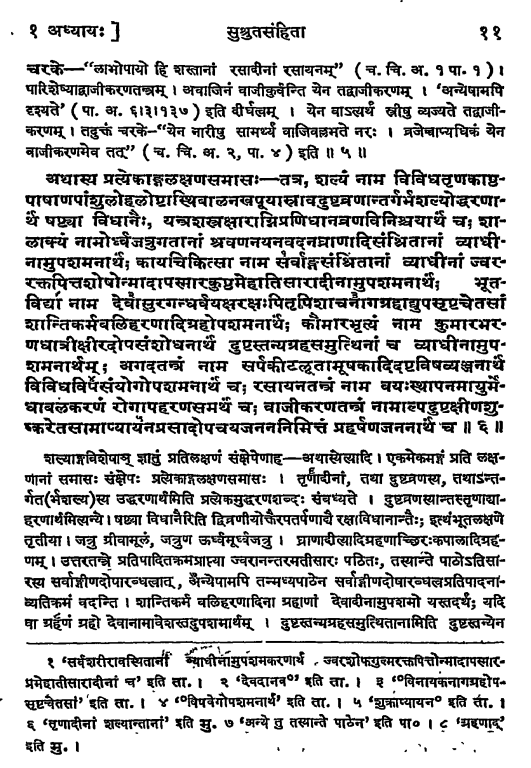
\includegraphics[draft=false,height=.9\textheight]{media/Bhanumati-page-11}
    \caption{A page of the 1939 \emph{Bhānumatī} edition, showing the variant 
        readings in 
        the 
        footnotes.}
    \label{bhanumati}
\end{figure}


\paragraph{For the Bhānumatī}

\begin{enumerate}
    \item A printed edition.  Covered the \emph{Bhānumatī} up to chapter Su.sū.40.
    The siglum was \dev{mu} for \emph{mudrita}.\footnote{\cite{sena-1886}.  
    The
    manuscript on which this edition was based is probably in the library of the
    Calcutta Sanskrit College, and described in \cite[v.\,X.1]{sast-1917}, which
    is not available to me.  See also \cite[IB, 495, n.\,57]{meul-hist} for
    mention of this manuscript.  The reference at \cite[217]{rao-sans} to CSCL
    accession number 97 in Bengali script may be this manuscript.}
    
    \item A manuscript in the India Office Library library provided through the
    Bhandarkar Oriental Research Institute in Pune.\footnote{At this time,
    manuscripts from Britain were routinely lent to scholars in India and vice
    versa.} This manuscript covered the \emph{Bhānumatī} b up to the end of the
    \emph{sūtrasthāna}.  The siglum was \dev{ha} for
    \dev{hastalikhita}.\footnote{\cite{PP109978}\\ 
    \MScite{London BL H. T. Colebrooke 908}
    (\href{panditproject.org/entity/109978/manuscript}{PanditProject \#109978},
    consulted on July 03, 2021).}
\end{enumerate}

\paragraph{For the Suśrutasaṃhitā}

\begin{enumerate}
    \item A palm leaf manuscript from Hemarājaśarman's personal
    library.\footnote{I.e., \MScite{Kathmandu NAK 5-333}.}  The siglum was
    \dev{tā} for \dev{tāḍapatra}.
    
    \item His own published edition. The siglum was \dev{ḍa} for 
    \dev{ḍalhaṇasaṃmataḥ
        pāṭhaḥ}.\footnote{\cite{vulgate}.  It is noteworthy that Ācārya refers to
    his 1938 edition as representing “the Ḍalhaṇa recension.”}
    
    \item Hārāṇacandra Cakravarti's published edition with his own
    commentary.\footcite{bhat-1917} The siglum was \dev{hā}.
\end{enumerate}
%
\subsubsection{Evaluation}

The main innovation of this publication was to present the only surviving part of
the commentary on the \SS\ by the great eleventh-century medical scholar
Cakrapāṇidatta, namely the \emph{Bhānumatī}.\footcite[IA, 374--375 and IB,
495--496]{meul-hist} A secondary purpose was to present the text of the
\emph{sūtrasthāna} as read in \MScite{Kathmandu NAK 5-333}, that had recently 
been
brought to the editors' attention. In their judgement, the Kathmandu manuscript
presented a text that was closer to what Cakrapāṇidatta had before him than the
text according to Ḍalhaṇa.   This was the first \SS\ edition in which Ācārya used
sigla to identify the sources from which variant readings were reported, so while
it has limitations, it for the first time enables us to get some idea of origins
of the text (see Figure~\ref{bhanumati}).

Ācārya noted in his introduction that the manuscripts containing the Ḍalhaṇa's
commentary all came together with the root-text of the \SS, and thus the main \SS\
text reflected the readings chosen by Ḍalhaṇa.  But the manuscripts of the
\emph{Bhānumatī} contained the commentary alone, without the root-text, and 
had
many explanations based on different readings of the root-text than those of
Ḍalhaṇa.  In many of these cases it was hard to know what the text that
Cakrapāṇidatta had before him. But Ācārya noted that Cakrapāṇidatta had a text
before him that had much in common with the text of the Nepalese
manuscript.\footnote{\cite[3--4]{acar-1939}.  See discussion by
\citet[7]{kleb-2021a}.}  

There is compelling evidence that Cakrapāṇidattas's \emph{Bhānumatī} 
commentary
once covered the whole text of the \SS.\footcite[IA, 375]{meul-hist}  The loss of
the rest of the work ranks amongst the greatest disasters in Āyurvedic
literature.  Remarkably, the whole \emph{Bhānumatī} may still have existed in the
early twentieth century. In 1903, Palmyr Cordier reported being privately informed
of a complete copy of the work in a personal manuscript collection in
Benares.\footcite[332]{cord-1903}
   
\subsection{Editorial Principles}
\subsubsection{Method}
The data for the critical edition comes from the witnesses of the Nepalese version, which are MS KL 699, NAK 5-333 and NAK 1-1079. Diplomatic transcriptions of SS.1.16 of these manuscripts have been created by researchers of the \href{https://sushrutaproject.org}{Suśruta Project}\space%\footnote{https://sushrutaproject.org, accessed 20/8/2021.} 
according to a subset of TEI Guidelines that has been formulated by Charles Li.\footnote{These guidelines are at \url{https://saktumiva.org/wiki/tei}, accessed 20/10/2021.} MS NAK 5-333 was transcribed first because its script is easy to read, the scans are clear, and it is the most complete of the manuscript witnesses. Then, MS KL 699 and MS NAK 1-1079 were transcribed. 

The diplomatic transcripts were uploaded to Charles Li's platform Saktumiva, which automatically collates them. An electronic text of the vulgate of the \SS, which was transcribed without the commentaries by Tsutomu Yamashita and Yasutaka Muroya on the basis of Ācārya's 1931 and 1938 Bombay editions,\footnote{This e-text is available on the SARIT website; \url{https://sarit.indology.info/susrutasamhita.xml?view=div}, accessed 20/8/2021.} has also been included in the collation. 

Saktumiva's automatic collation function standardises punctuation and orthographic variants according to filters which can be turned off or on. These filters enable the editors to ignore \emph{daṇḍa}s, numbers and \emph{puṣpikā}s in the transcripts, as well as orthographic variants, such as \emph{ba} and \emph{va}, certain germinated consonants, and \emph{visarga} variants. On the basis of the automatic collation, Jason Birch created a provisional edition of SS.1.16, which the project's researchers read together at weekly seminars. Manuscript images were routinely checked to verify the transcripts, particularly when a reading was uncertain; the commentaries of Cakrapāṇidatta and Ḍalhaṇa were read, and variant readings reported by these commentators were included in notes to the edition. Also, various reference books were consulted, such as the  \citet{josi-maha,nadk-1954} and \citet{meul-hist}, to elucidate the meaning of technical terms and identify relevant information in other medical works. 

An initial draft of the translation and many annotations were written by Dominic Wujastyk during the seminars as the Project researchers discussed the text's meaning. The transcripts, provisional edition and translation were uploaded to the project's repository at Github on a weekly basis. Therefore, the project's work has been publicly available as it evolves. The following software tools have been selected by Wujastyk for the procedures described above: 

\begin{enumerate}
    \item
    \href{https://www.oxygenxml.com.}{oXygen XML editor} (which has plugins for Github and TEI, and can validate the code).%\footnote{https://www.oxygenxml.com.}
    
       \item
        \href{http://saktumiva.org.}{Saktumiva} (a platform for producing and publishing critical editions of Sanskrit texts).%\footnote{http://saktumiva.org.}
        \item
         \href{https://tst.hypotheses.org/1738.}{Quick Palaeographer} (a browser-based tool for reading MS images and developing a catalogue of character shapes).%\footnote{https://tst.hypotheses.org/1738.}

        \item
         \href{https://filezilla-project.org.}{Filezilla} (document transfer to Saktumiva).%\footnote{https://filezilla-project.org.}       
        \item
         \href{https://github.com.}{Github} (document sharing, security and versioning).%\footnote{https://github.com.}   
        \item
          \href{https://www.latex-project.org.}{LaTeX} (document preparation).%\footnote{https://www.latex-project.org.}  
         \item
           \href{https://qdpm.net.}{qdpm} (project management).%\footnote{https://qdpm.net.}  
          
\end{enumerate}

\subsubsection{Stemma}
The data from transcripts collated by Saktumiva can be exported as a FASTA file 
and aligned according to characters, syllables or words by a program called 
Helayo. The resulting NEXUS file can be read by phylogenetics software to build a 
stemmatic tree.\footnote{This process is discussed in greater detail by Charles Li 
at \url{https://chchch.github.io/sanskrit-alignment/docs/index.html\#tree}, 
accessed 21/8/2021.} This procedure was done with transcripts of several 
chapters of the Nepalese witnesses, and the results confirmed the editors' provisional stemmatic hypothesis that 
K and H are more closely related to one another than K and N.\footnote{See 
section `Features of the Manuscript Transmission' for further discussion of this.} 
Given the early date of K and the small number of other surviving witnesses of the 
Nepalese version, the relationship between the manuscripts at our disposal is 
reasonably clear and, in the case of SS.1.16, the manuscript data was largely 
confined to N and H owing to a missing folio of K. The challenge of editing has 
been to repair the text in the places where it has become corrupt in the
available witnesses. 

\subsubsection{The Edition and Apparatus}
The critical edition of SS.1.16 in this article retains many of the peculiarities of MS KL 699 because the editors have endeavoured to present to the reader a text that is very similar to the one transmitted in the region of Nepal in the ninth century. Therefore, the Sanskrit has been standardised as minimally as possible and, although the text has been corrected and repaired wherever it seemed corrupt, it has not been normalized or conventionalized to the extent of many modern editions of Sanskrit works. 

The editors have assumed that the authors of the Nepalese \SS\ were familiar with Pāṇinian Sanskrit and, although there are some non-standard spellings and grammatical forms in the text, there are very few instances of hyper-Sanskritization, Buddhist-hybrid Sanskrit or Epic forms that would suggest that this assumption is unreasonable. Therefore, the editors of SS.1.16 have opted to retain some unusual features of the Sanskrit in MS KL 699 when they are grammatically correct. For example, in external \emph{sandhi}, the class nasal is usually used at the end of a word instead of an \emph{anusvāra} (e.g.,1.16.3, \emph{°vācanan dhātry°}), although the \emph{anusvāra} is sometimes used (1.16.15, \emph{udakaṃ dhānyāmla°}). In most cases, the consonant following a \emph{repha} is doubled, but this is not always the case.\footnote{Examples of the germination of consonants are \emph{karṇṇa} (1.16.1 ff), \emph{muhūrtta} (1.16.2), \emph{pūrvva} (1.16.2), \emph{gandharvva} (1.16.5), \emph{°mūlair mmadhu°} (1.16.5), \emph{vartti} (1.16.6) and \emph{punar vvidhyet} (1.16.6). Examples where it does not occur in 1.16 are  \emph{°ārtham} (1.16.8,19), \emph{kuryāt} (1.16.16, 32), \emph{°pālir vallūra°} (1.16.10); \emph{°pālir vyāyojimaḥ} (1.16.10) and \emph{dīrghaika°} (1.16.10).} Since these inconsistencies seem inherent to the transmission of the text and may have even been authorial, the critical edition reflects them as they occur in K and, when the testimony of K is not available, the witness most similar to K, which is H.


% This is not always consistent: °ārtham (1.16.8,19), kuryāt (1.16.16, 32), °pālir vallūra°  (1.16.10); °pālir vyāyojimaḥ (1.16.10); dīrghaika° (1.16.10).

% external sandhi
% A tendency to favour the use of the class nasal instead of ṃ (e.g.,1.16.3 svastivācanan dhātryaṅke), although ṃ is sometimes used (1.16.15 udakaṃ dhānyāmla°)

% germination of consonants after a repha, even between words.
% karṇṇa (1.16.1 ff), muhūrtta (1.16.2), pūrvva (1.16.2), gandharvva (1.16.5), °mūlair mmadhu° (1.16.5), vartti (1.16.6), punar vvidhyet (1.16.6), °pālir nnirvvedhimaḥ
% This is not always consistent: °ārtham (1.16.8,19), kuryāt (1.16.16, 32), °pālir vallūra°  (1.16.10); °pālir vyāyojimaḥ (1.16.10); dīrghaika° (1.16.10).

The Nepalese manuscripts often have an \emph{anusvāra} before a \emph{daṇḍa} at the end of a sentence or verse. Whether these \emph{anusvāra}s should be changed to the consonant \emph{m} is a moot question because there is no Pāṇinian concept of `end-of-sentence' and his rules on \emph{sandhi} are contingent on the close contact of  sounds (\emph{saṃhitā})\q{refs?}. However, it is reasonable to assume that at the end of a verse, paragraph or sentence the speakers would have paused for breath or thought, in which case \emph{sandhi} should be applied and a final \emph{anusvāra} or class nasal of the following consonant changed to \emph{m}.  Nonetheless, this remains an assumption about how the text would be pronounced. Therefore, the insertion of \emph{daṇḍa}s and changing \emph{anusvāra}s to \emph{m} before them in the critical edition are subjective decisions by the editors. The scribal use of \emph{daṇḍa}s and \emph{anusvāra}s in the Nepalese manuscripts can be seen in the digital edition if one switches off the filters for ignoring \emph{daṇḍa}s and final \emph{anusvāra} variants. 

Unconventional spellings and grammatical forms have been retained and noted in the annotations to the translation. However, the editors have corrected scribal errors and repaired corruptions in the transmitted text with conjectures wherever possible. Therefore, although the edition retains many of the peculiarities of the Nepalese manuscripts, it is not a diplomatic transcript or a hybrid of diplomatic and critical editing because the features of the transmitted text have been retained or changed deliberately, and the reasons for doing so are given in either the introduction or, in more specific cases, the annotations to the translation.

\subsubsection{Printed Edition}
The editors intend to produce both printed and digital editions of the Nepalese \SS. Since the print and digital environments differ markedly, each edition has its own format. The printed edition of SS.1.16 in this article has a positive apparatus, that is to say, the testimony of every witness is recorded for the lemma and variants. The following entry is an example of the apparatus' syntax:
\begin{quote}
pratanuṃ K ]  pratanū N, H tataḥ A
\end{quote}
This entry means that the editors have chosen to read \emph{pratanuṃ}, which is the reading of K. Instead of \emph{pratanuṃ}, witnesses N and H have \emph{pratanū} and A has \emph{tataḥ}. In prose passages, the lemma and variants consist of corresponding words and, in verses, corresponding syllables. Conjectures by the editors are indicated by the abbreviation \emph{conj}. Omissions and suppletions in the witnesses are indicated by \textsc{[OM]} and \textsc{[ADD]} next to the siglum. There are separate layers of footnotes in the printed edition for testimonia and notes. The testimonia mainly consists of the variant readings noted by the commentators Cakrapāṇidatta and Ḍalhaṇa. Those known to Gayadāsa will be added in future publications. The notes include the additional passages and verses in the version known to Ḍalhaṇa and large omissions in the witnesses. Reasons for editorial decisions and notes on peculiarities in the text have been included in the annotations to the translation.

\subsubsection{Digital Edition}
Instructions for reading the digital edition have been provided by Charles Li on \href{https://saktumiva.org/wiki/users}{Saktumiva}. In brief, the reader is able to generate the apparatus by choosing a base text and one or more of the other witnesses. The reader can also chose to hide or ignore in varying degrees TEI tags, punctuation and orthographical variants in the transcript of each witness. On the right side of the text, the digital edition displays an apparatus that is negative in so far as the lemma and its witnesses are not included. This apparatus truncates variants wherever possible. 

\begin{figure}[h]
    \centering
    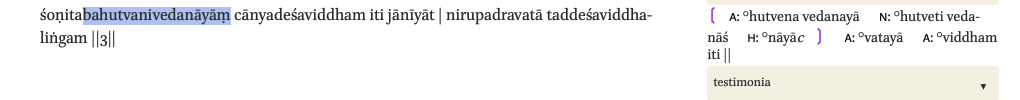
\includegraphics[draft=false,scale=.375]{media/SS.1.16}
    \caption{The digital edition of SS.1.16.3}
    \label{SS.1.16}
\end{figure}

For example, as seen in Figure 2, the apparatus for the highlighted words \emph{bahutvanivedanāyāṃ} is on the right side between the purple square brackets. This entry means that the editors have chosen to read \emph{°bahutvanivedanāyāṃ}, which is the reading of K, whereas A has \emph{°bahutvena nivedanayā}, N \emph{°bahutveti vedanāś} and H \emph{°bahutvanivedanāyāc}. The final \emph{c} in the reading of H is italicised because it has been marked by the transcriber as unclear.

A positive apparatus is available if one highlights with the cursor one or more words, and even entire passages or verses, and clicks on the collapsed menu icon. 
As seen in Figure 3, the positive apparatus of \emph{°bahutvanivedanāyāṃ} appears in a pop-up window in which the lemma and variants are aligned according to letters, and the variations are highlighted in yellow.

\begin{figure}[h]
    \centering
    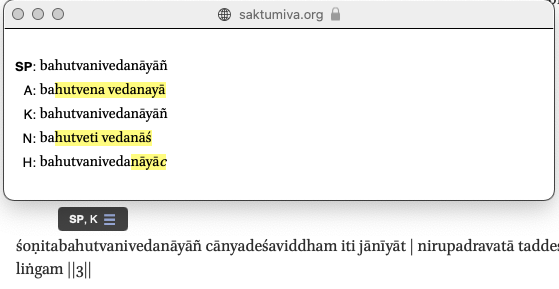
\includegraphics[draft=false,scale=.5]{media/SS.1.16.positive}
    \caption{The digital edition of SS.1.16.3}
    \label{SS.1.16}
\end{figure}

In both the negative and positive apparatuses of the digital edition, the reader must infer conjectures and corrections by the editors. Testimonia and notes are in the apparatus on the right side of the text. 




